% \documentclass[twocolumn, 10pt,a4j]{jsarticle}
\documentclass[10pt,a4j]{jsarticle}
\usepackage{amsmath}
\usepackage[dvipdfmx]{graphicx}
\usepackage{url}
\usepackage{listings,jlisting} %日本語のコメントアウトをする場合jlistingが必
\usepackage{here}

\lstset{
  basicstyle={\ttfamily},
  identifierstyle={\small},
  commentstyle={\smallitshape},
  keywordstyle={\small\bfseries},
  ndkeywordstyle={\small},
  stringstyle={\small\ttfamily},
  frame={tb},
  breaklines=true,
  columns=[l]{fullflexible},
  numbers=left,
  xrightmargin=0zw,
  xleftmargin=3zw,
  numberstyle={\scriptsize},
  stepnumber=1,
  numbersep=1zw,
  lineskip=-0.5ex
}


% プリアンブル
\title{\vspace{-2.5cm}ロボットの基礎}
\author{1610581 堀田 大地}
\begin{document}
\renewcommand{\baselinestretch}{0.90}
\maketitle{}
\section{目的}
% 目的
バレタイズ作業のプログラムを行い,それを動作させることを通してロボットの操作方法,メカニズム,
運動学,制御法などに関する理解を深める.

\section{システム}
% 原理
  \subsection{ロボットアーム}
  % ロボットアーム
  本実験では三菱電機のロボットRV-2SDを用いた.
  RV-2SDは6軸多関節ロボットであり,各関節はベースから順にウエスト,ショルダ,エルボ,リストツイスト,
  リストピッチ,リストロールとである.各関節はハーモニックドライブ,タイミングベルトを介してACモータにより
  鼓動される.

  \subsection{電動ハンド}
  % 電動ハンド
  ロボットアームにTAIYO製の電動ハンドESG1-FT-2840を装着して対象物の把持を行う.
  このハンドは2爪の平行グリッパによって把持を行い,グリッパはモータとボールねじを利用して駆動している.
  また,ハンドには絶対位置エンコーダーではなく相対位置エンコーダが搭載されているため,ハンドはアームと
  異なり,電源を入れるたびに原点出しの準備動作が必要となる.

  \subsection{コントローラ}
  % コントローラ
  コントローラはロボットの制御に使用するプログラムを実行し,制御時に必要な各種計算(運動学計算や
  逆運動学計算)を行う装置である.
  本実験で使用するコントローラはTCP/IP通信でパーソナルコンピュータに接続されており,PCとの間で
  プログラムの送受信を行い,プログラムの選択・実行などをPC側から行うことができる.

  \subsection{ティーチングボックス}
  % ティーチングボックス
  ティーチングボックスは,ロボットアームに座標を教示するための装置である.

\section{手順}
% 内容と手順
  \subsection{教示}
  % 教示
  ロボットにバレタイズ作業を行わせるために,ティーチングボックス(TB)を用いて各ポジションの教示を行った.
  バレタイズとは,卵のパックのような容器に物体を指定した順番で,適当な位置に置く作業のことである.

  \subsection{教示のための準備}
  % 教示のための準備
  \begin{enumerate}
    \item コントローラの電源を入れ,MODE切替スイッチ"MANUAL"にした. \\
    \item TBの"[TB ENABLE]スイッチ"を押し点灯する状態にした. \\
    \item "[EXE]キー"を2回押し,メインメニューが表示されたら,カーソルを"1.管理・編集"に合わせ,
      "[EXE]キー"を押して選択した. \\
    \item "SAMPLE2"にカーソルを合わせ,"編集"を選択した. \\
    \item プログラムを開いたら,"FUNCTIONキー"を2回押してファンクションメニューを切り替え,
      "切替"を選択した. \\
    \item "\verb|<|位置\verb|>|モード"が開かれるので,教示したいポイントまでアームを移動させ,ファンクションメニュー
      を1回切り替えて,"教示"を選択して教示を行った.
  \end{enumerate}

  \subsection{ロボットアームの動作}
  % ロボットアームの動作
  TB背面の"イネーブルスイッチ"を押しながら,"[SERVO]キー"を押しサーボモータの電源を入れた.
  次に"[JOG]キー"を押してジョグモードに切り替え,この状態で"[ジョグ操作]キー"を操作することで
  ロボットアームを動かした.

  \subsection{ハンドの動作}
  % ハンドの操作
  "[HAND]キー"を押してハンド操作モードに変更した."原点"を原点チェックボックスにチェックが入るまで
  長押しして初期化を行った後,ハンド操作を行った.

  \subsection{教示の位置}
  % 教示の位置
    \begin{enumerate}
      \item ボルトを掴む位置 \\
        \begin{enumerate}
          \item TBでボルトをハンドの中心でつかめる位置までロボットハンドを動かした. \\
          \item ハンドを開いたままポジションを教示した. \\
          \item ハンドを閉じ,ボルトをつかみ,持ち上げた.
        \end{enumerate}
      \item スイッチを押す位置 \\
        \begin{enumerate}
          \item ボルトを掴んだ状態で,ボタンスイッチを押せるような位置を決めた. \\
          \item ポジションを記憶させ,ボルトを上に回避させた. \\
        \end{enumerate}
      \item ボルトを落とす位置 \\
        \begin{enumerate}
          \item バレットにある10個の穴の位置をロボットに教えるために,4隅の上でボルトを落とせる
            位置を教示した.
        \end{enumerate}
    \end{enumerate}

  \subsection{実行}
  % 実行
    \begin{enumerate}
      \item 制御用プログラム"RT ToolBox2"を起動した. \\
      \item ワークスペース"test3"を開く. \\
      \item コントローラのモードを"AUTOMATIC"にし,オンラインモードに切り替えた. \\
      \item オンラインのディレクトリを開いた. \\
      \item 実行するプログラム上で右クリックし,"デバッグ状態で開く"を選択した. \\
      \item サーボの電源を入れ,プログラム実行ボタンを選択する. \\
    \end{enumerate}

\section{結果}
% 実験結果
  \subsection{パターン4}
  % パターン4
  図1のパターンのバレンタイズを実行するプログラムを作成した.
  作成したプログラムを示す.

    \begin{figure}[H]
      \centering
      % 図1
      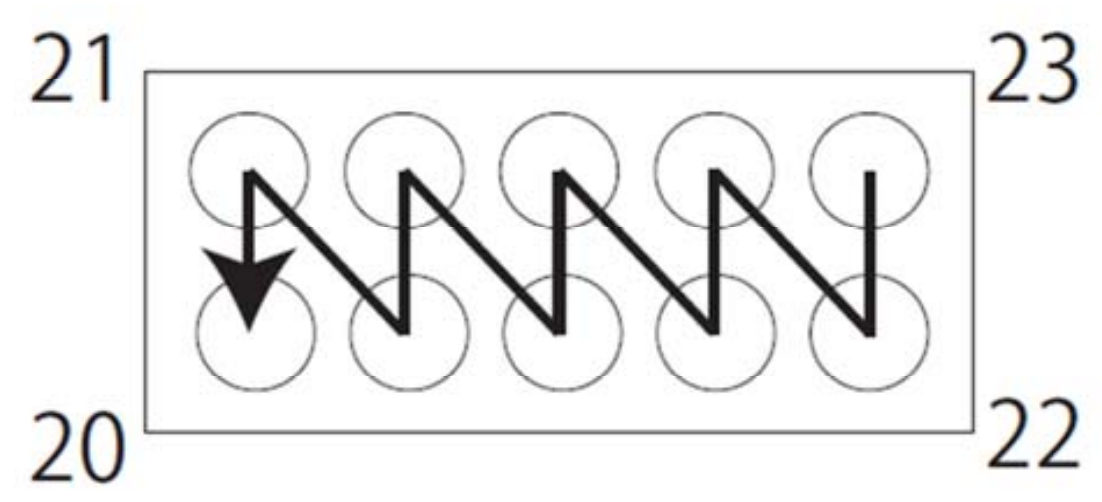
\includegraphics[width=7cm]{../img/pattern4.png}
      \caption{パターン4のバレンタイズ}
    \end{figure}

  \begin{lstlisting}[caption=パターン4のソースコード, label=p4_txt]
    1 Spd 20 速度を設定.
    2 If M_EHOrg=0 Then 原点復帰未完了のとき.
    3    EHOrg 1 ハンド1復帰.
    4    Wait M_EHOrg=1 ハンド1原点復帰完了待ち.
    5 EndIf If終了.
    6 For MJ=0 To 4 変数MJを0~4まで+1ずつ増加させながら反復.
    7    For MI=0 To 1 変数MIを0~4まで+1ずつ増加させながら反復.
    8      PTemp=P23 変数PTempにP23を代入.
    9      PTemp=PTemp - PV*MJ - PW*MI PTempに右辺の計算結果を代入.
    10     *LBL1 Mov P1, -30 ラベル1:ワークをつかむ位置P1の上空30mmへ関節補間移動.
    11     EHOpen 1, 50, 30 ハンド1を50%の速度と30%の力で開く.
    12     Wait M_EHBusy=0 ハンドの完了動作を待つ.
    13     Mvs P1 ワークをつかむ位置P1へ直線補間移動.
    14     EHClose 1, 50, 30 ハンド1を50%の速度と30%の力で閉じる.
    15     Wait M_EHBusy=0 ハンドの完了動作を待つ.
    16     Mvs P1, -15 ワークをつかむ位置P1の上空15mmへ直線補間移動.
    17     Mov P1, -70 ワークをつかむ位置P1の上空70mmへ関節補間移動.
    18     Mov P3, -20 スイッチを押す位置P3の上空20mmへ関節補間移動.
    19     Def Act 1, M_In(31)=1 GoTo *LBL2 優先番号1の割り込み処理を定義.入力信号31の信号が1になったら,ラベル2の行にジャンプする.
    20     Act 1=1 優先番号1の割り込み処理.
    21     Mvs P3 スイッチを押す位置P3へ直線補間移動.
    22     Act 1=0 優先番号1の割り込み処理を禁止.
    23     Mvs P3, -20 スイッチを押す位置P3の上空20mmへ直線補間移動.
    24     Mov PErr スイッチを押せなかったときに行く位置PErrへ関節補間移動.
    25     EHOpen 1, 50, 30 ハンド1を50%の速度と30%の力で開く.
    26     Wait M_EHBusy=0 ハンドの動作完了を待つ.
    27     GoTo *LBL1 LBL1へGoTo.
    28     *LBL2  Act 1 = 0 ラベル2,優先番号1の割り込み処理を禁止.
    29     Mvs P3, -20 スイッチを押す位置P3の上空20mmへ直線補間移動.
    30     Mov PTemp, -90 PTempの上空90mmへ関節補間移動.
    31     Mov PTemp, -10 PTempの上空10mmへ関節補間移動.
    32     EHOpen 1, 30, 30 ハンド1を速度50%,力30%で開く.
    33     Wait M_EHBusy=0 ハンドの動作完了を待つ.
    34     Mov PTemp, -50 Ptempの上空50mmへ関節補間移動.
    35   Next MI 7行目へ戻る.
    36 Next MJ 6行目へ戻る.
    37 End プログラム終了.
    PTemp=(+424.52,-31.92,+172.64,-171.43,-12.49,-94.16,+0.00,+0.00)(7,0)
    P20=(+403.76,+138.90,+166.76,+175.18,-1.73,-96.51,+0.00,+0.00)(7,0)
    PV=(+0.00,-48.26,+0.00,+0.00,+0.00,+0.00,+0.00,+0.00)(0,0)
    PW=(+46.12,+0.00,+0.00,+0.00,+0.00,+0.00,+0.00,+0.00)(0,0)
    P1=(+365.96,-226.66,+156.70,-165.67,+4.82,-167.50,+0.00,+0.00)(7,0)
    P3=(+260.04,+25.14,+248.15,+179.30,-1.25,-96.72,+0.00,+0.00)(7,0)
    PErr=(+460.54,-133.35,+184.36,+177.63,-4.42,-134.98)(7,0)
    P0=(+375.14,-11.15,+299.92,-179.07,-4.90,-166.26)(7,0)
    P21=(+450.71,+141.59,+169.03,+174.36,-0.79,-84.77,+0.00,+0.00)(7,0)
    P22=(+408.24,-45.75,+166.76,+175.19,-1.72,-96.51,+0.00,+0.00)(7,0)
    P23=(+450.46,-47.81,+169.03,+174.36,-0.80,-84.82,+0.00,+0.00)(7,0)
  \end{lstlisting}

  \subsection{パターン6}
  % パターン6
  図2のパターンのバレンタイズを実行するプログラムを作成した.
  作成したプログラムを示す.

    \begin{figure}[H]
      \centering

      % 図1
      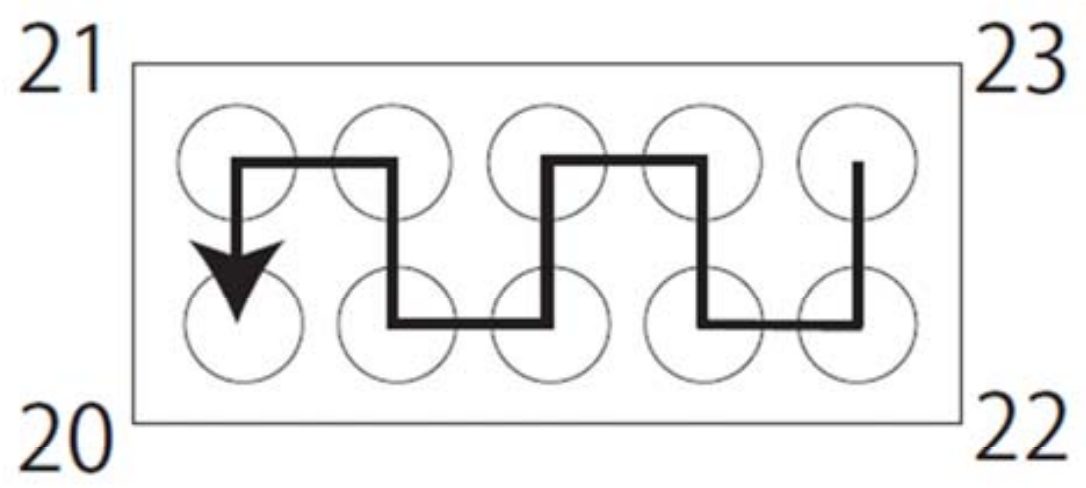
\includegraphics[width=7cm]{../img/pattern6.png}
      \caption{パターン6のバレンタイズ}
    \end{figure}

  \begin{lstlisting}[caption=パターン4のソースコード, label=p4_txt]
    1 Spd 20 速度を設定.
    2 If M_EHOrg=0 Then 原点復帰未完了のとき.
    3    EHOrg 1 ハンド1復帰.
    4    Wait M_EHOrg=1 ハンド1原点復帰完了待ち.
    5 EndIf If終了.
    6 MI = 0 MI = 0を代入.
    7 MJ = 0 MJ = 0を代入.
    8 For a=0 To 9 変数aを0~9まで+1ずつ増加.
    9    PTemp=P23 変数PTempにP23を代入.
    10   PTemp=PTemp - PV*MJ - PW*MI PTempに右辺の計算結果を代入.
    11   *LBL1 Mov P1, -30	ラベル1:ワークをつかむ位置P1の上空30mmへ関節補間移動.
    12   EHOpen 1, 50, 30 ハンド1を50%の速度と30%の力で開く.
    13   Wait M_EHBusy=0 ハンドの完了動作を待つ.
    14   Mvs P1 ワークをつかむ位置P1へ直線補間移動.
    15   EHClose 1, 50, 30 ハンド1を50%の速度と30%の力で閉じる.
    16   Wait M_EHBusy=0 ハンドの完了動作を待つ.
    17   Mvs P1, -15 ワークをつかむ位置P1の上空15mmへ直線補間移動.
    18   Mov P1, -70 ワークをつかむ位置P1の上空70mmへ関節補間移動.
    19   Mov P3, -20 スイッチを押す位置P3の上空20mmへ関節補間移動.
    20   Def Act 1, M_In(31)=1 GoTo *LBL2 優先番号1の割り込み処理を定義.入力信号31の信号が1になったら,ラベル2の行にジャンプする.
    21   Act 1=1 優先番号1の割り込み処理.
    22   Mvs P3 スイッチを押す位置P3へ直線補間移動.
    23   Act 1=0 優先番号1の割り込み処理を禁止.
    24   Mvs P3, -20 スイッチを押す位置P3の上空20mmへ直線補間移動.
    25   Mov PErr スイッチを押せなかったときに行く位置PErrへ関節補間移動.
    26   EHOpen 1, 50, 30 ハンド1を50%の速度と30%の力で開く.
    27   Wait M_EHBusy=0 ハンドの動作完了を待つ.
    28   GoTo *LBL1 LBL1へGoTo.
    29   *LBL2  Act 1 = 0 ラベル2,優先番号1の割り込み処理を禁止.
    30   Mvs P3, -20 スイッチを押す位置P3の上空20mmへ直線補間移動.
    31   Mov PTemp, -90 PTempの上空90mmへ関節補間移動.
    32   Mov PTemp, -10 PTempの上空10mmへ関節補間移動.
    33   EHOpen 1, 30, 30 ハンド1を速度50%,力30%で開く.
    34   Wait M_EHBusy=0 ハンドの動作完了を待つ.
    35   Mov PTemp, -50 Ptempの上空50mmへ関節補間移動.
    36   MK = MI + MJ MJにMI+MJを代入.
    37   M = MK Mod 2 MにMKを2で割った余りを代入.
    38   IF M == 0 Then M=0のとき.
    39     IF MI == 1 Then MI=1のとき.
    40       MI = MI - 1 MIから1を引く.
    41     Else MI=1じゃないとき.
    42       MI = MI + 1 MIに1を足す.
    43     Endif If終了.
    44   Else M=0じゃないとき.
    45     MJ = MJ + 1 MJに1を足す.
    46   Endif if終了.
    47   Next a 8に戻ってaに1を足す.
    48 End
    PTemp=(+424.52,-31.92,+172.64,-171.43,-12.49,-94.16,+0.00,+0.00)(7,0)
    P20=(+403.76,+138.90,+166.76,+175.18,-1.73,-96.51,+0.00,+0.00)(7,0)
    PV=(+0.00,-48.26,+0.00,+0.00,+0.00,+0.00,+0.00,+0.00)(0,0)
    PW=(+46.12,+0.00,+0.00,+0.00,+0.00,+0.00,+0.00,+0.00)(0,0)
    P1=(+365.96,-226.66,+156.70,-165.67,+4.82,-167.50,+0.00,+0.00)(7,0)
    P3=(+260.04,+25.14,+248.15,+179.30,-1.25,-96.72,+0.00,+0.00)(7,0)
    PErr=(+460.54,-133.35,+184.36,+177.63,-4.42,-134.98)(7,0)
    P0=(+375.14,-11.15,+299.92,-179.07,-4.90,-166.26)(7,0)
    P21=(+450.71,+141.59,+169.03,+174.36,-0.79,-84.77,+0.00,+0.00)(7,0)
    P22=(+408.24,-45.75,+166.76,+175.19,-1.72,-96.51,+0.00,+0.00)(7,0)
    P23=(+450.46,-47.81,+169.03,+174.36,-0.80,-84.82,+0.00,+0.00)(7,0)

  \end{lstlisting}

\section{課題}
% 課題

  \subsection{必須課題1}
    % 必須課題1
    順運動学では各関節状態からロボットの手先の位置・姿勢が一意な解として求まるのに対し,
    逆運動学では目的とするロボットの手先位置・姿勢から各関節の状態が一意に求まらないことを説明する.
    \par まず,順運動学について図3の解を求める.
      \begin{figure}[H]
        \centering
        % 図1
        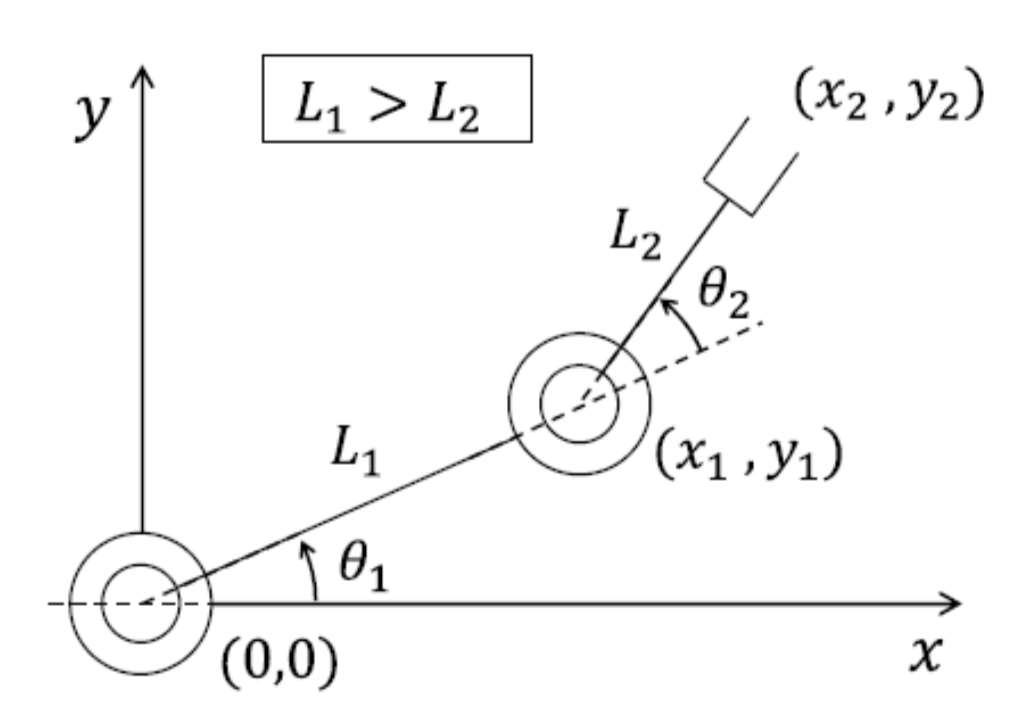
\includegraphics[width=7cm]{../img/ziyuudo2_robo_arm.png}
        \caption{パターン4のバレンタイズ}
      \end{figure}
    Eq.1,2より$\theta_{1}$と$\theta_{2}$が求まれば解が一つに定まる.なので,順運動学では各関節の状態から
    ロボットの手先の位置・姿勢が一意な解として求まる.
      \begin{eqnarray}
        (x_{1}, y_{1}) &=& (L_{1}\cos\theta_{1}, L_{1}\sin\theta_{1}). \\
        (x_{2}, y_{2}) &=& (L_{1}\cos\theta_{1} + L_{2}\cos{(\theta_{1} + \theta_{2})}, L_{1}\sin\theta_{1} + L_{2}\sin{(\theta_{1} + \theta_{2})}).
      \end{eqnarray}

    \par 次に,逆運動学についての解を求める.Eq.3,4として,Eq.2の各成分の二乗の和を取るとEq.5になる.
    よって,Eq.6となる.
      \begin{eqnarray}
        x_{2} &=& x. \\
        y_{2} &=& y. \\
        x^{2} + y^{2} &=& {L_{1}}^{2} + {L_{2}}^{2} + 2L_{1}L_{2}\cos\theta_{2}. \\
        \theta_{2} &=& \cos^{-1}\left[ \frac{(x^2 + y^2) - (L_{1}^2 + L_{2}^2)}{2L_{1}L_{2}} \right].
      \end{eqnarray}
    さらに,Eq.2について,Eq.7のように変形した.また,Eq.7の両辺に
    \[
      \left[\begin{array}{cc}
        L_{1} + L_{2}\cos\theta_{2} & -L_{2}\sin\theta_{2} \\
        L_{2}\sin\theta_{2} & L_{1} + L_{2}\cos\theta_{2}
        \end{array}
      \right]^{-1}
    \]
    を左からかけると,Eq.8となった.
    これより,Eq.9,10が導出される.つまり,Eq.11より,$x$,$y$の値が求まっても
    解が二つ出てくることより,解が一意に定まらない.
    よって,逆運動学では目的とするロボットの手先位置・姿勢から各関節の状態が一意に求まらない.
      \begin{eqnarray}
        \left[
          \begin{array}{c}
            x \\
            y
          \end{array}
        \right] &=& \left[
                        \begin{array}{cc}
                          L_{1} + L_{2}\cos\theta_{2} & -L_{2}\sin\theta_{2} \\
                          L_{2}\sin\theta_{2} & L_{1} + L_{2}\cos\theta_{2}
                        \end{array}
                      \right] 
                        \left[
                          \begin{array}{c}
                              \cos\theta_{1} \\
                              \sin\theta_{1}
                          \end{array}
                        \right]. \\
        \left[
          \begin{array}{c}
            \cos\theta_{1} \\
            \sin\theta_{1}
          \end{array}
        \right] &=& \left[
                        \begin{array}{cc}
                          L_{1} + L_{2}\cos\theta_{2} & -L_{2}\sin\theta_{2} \\
                          L_{2}\sin\theta_{2} & L_{1} + L_{2}\cos\theta_{2}
                        \end{array}
                      \right]^{-1}
                        \left[
                          \begin{array}{c}
                              x \\
                              y
                          \end{array}
                        \right]. \\
        \tan\theta_{1} &=& \frac{L_{1} + L_{2}\cos\theta_{2}y - (L_{2}\sin\theta_{2}x)}{L_{1} + L_{2}\cos\theta_{2}y + (L_{2}\sin\theta_{2}x)}. \nonumber \\
        &=& \frac{\frac{y}{x} - \frac{L_{2}\sin\theta{2}}{L_{1} + L_{2}\cos\theta_{2}}}{1 + \frac{y}{x}・\frac{L_{2}\sin\theta_{2}}{L_{1} + L_{2}\cos\theta_{2}}}. \\
        \theta_{1} &=& \tan^{-1}\left(\frac{y}{x}\right) - \tan^{-1}\left(\frac{\sqrt{4L_{1}^{2}L_{2}^{2} - {(x^{2} + y^{2}) - (L_{1}^{2} + L_{2}^{2})}^{2}}}{2L_{1}^{2} + (x^{2} + y^{2}) - (L_{1}^2 + K_{2}^2)     }\right).
      \end{eqnarray}


\subsection{必須課題2}
% 必須課題2
  直線補間動作の時,ロボットが実行可能な経路を生成できなく例を考える.
  図7のロボットアームにおいて,原点を中心とした半径$L_{1} - L_{2}$の円の領域には長さ$L_{2}$
  の腕は入ることはできない.なぜなら,本体にぶつかるからだ.よって,実行不可能な経路の例として,
  図の座標$(x_{2}, y_{2})$を始点にして,終点を$(-x_{2}, y_{2})$にした場合の経路である.

\begin{thebibliography}{3}
\bibitem{}ロボットの基礎 授業テキスト
\end{thebibliography}
\end{document}